%        File: hw2.tex
%     Created: Sun Oct 2 05:00 PM 2013 E
% Last Change: Sun Oct 2 05:00 PM 2013 E
%
\documentclass[a4paper]{report}

\title{HW 3}
\author{Delos Chang}
\date{}

\usepackage{amsmath, amsthm, amssymb, fancyhdr, tikz}
\usetikzlibrary{arrows}
\newcommand{\justif}[2]{&{#1}&\text{#2}}

\pagestyle{fancy}
\rhead{HW 3:  Delos Chang (help from Prof.)}
\begin{document}
  \begin{enumerate}
    %&=& &=& &=& &=& &=& &=& &=& &=& &=& &=& &=& &=& &=& &=& &=& =
    % Question 1 
    %&=& &=& &=& &=& &=& &=& &=& &=& &=& &=& &=& &=& &=& &=& &=& =
    \item
      **In a tree, for any two nodes $a$ and $b$, a unique path exists from $a$ to $b$.

      - Run BFS from any arbitrary node $u$ in the graph $T=(V,E)$. Mark the node $v$ with the highest discovery time in the BFS, 
      i.e. the node that is discovered last. $v$ must be a leaf node. 

      - Run BFS starting from node $v$. Mark the node $v_2$ with the highest discovery time in the BFS i.e. the node that is discovered last. 
      $\delta(v,v_2)$ is the diameter of the tree $T$. 




    %&=& &=& &=& &=& &=& &=& &=& &=& &=& &=& &=& &=& &=& &=& &=& =
    % Question 2 
    %&=& &=& &=& &=& &=& &=& &=& &=& &=& &=& &=& &=& &=& &=& &=& =
    \par
    \bigskip

    \item
      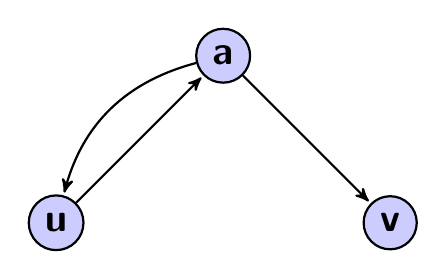
\begin{tikzpicture}[->,>=stealth',shorten >=1pt,auto,node distance=3cm,
        thick,main node/.style={circle,fill=blue!20,draw,font=\sffamily\Large\bfseries}]

        \node[main node] (1) {a};
        \node[main node] (2) [below left of=1] {u};
        \node[main node] (4) [below right of=1] {v};

        \path[every node/.style={font=\sffamily\small}]
        (1) edge node [left] {} (4)
        edge [bend right] node[left] {} (2)
        (2) edge node [right] {} (1);
      \end{tikzpicture}

      Consider a DFS run on the above counterexample directed graph $G$ starting from $a$.  
      There is clearly a path from $u$ to $v$ through $a$ (u-a-v).

      \begin{center}
        \begin{tabular}{ l | c | r }
          \hline
            & $d$ & $f$ \\ \hline
          $a$ & 1 & 6 \\
          $v$ & 4 & 5 \\
          $u$ & 2 & 3 \\
          \hline  
        \end{tabular}
      \end{center}

      The table shows that $d[u]=2$ and $d[v]=4$, thus $d[u] < d[v]$.

      $v$, however, is not a descendant of $u$ in the depth-first forest produced because the tree edges 
      in the depth-first forest are: $(a,u)$ and $(a,v)$. 

    %&=& &=& &=& &=& &=& &=& &=& &=& &=& &=& &=& &=& &=& &=& &=& =
    % Question 3 
    %&=& &=& &=& &=& &=& &=& &=& &=& &=& &=& &=& &=& &=& &=& &=& =
    \par
    \bigskip

    \item
      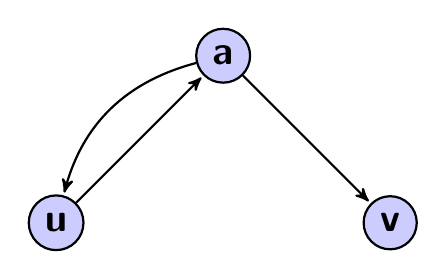
\begin{tikzpicture}[->,>=stealth',shorten >=1pt,auto,node distance=3cm,
        thick,main node/.style={circle,fill=blue!20,draw,font=\sffamily\Large\bfseries}]

        \node[main node] (1) {a};
        \node[main node] (2) [below left of=1] {u};
        \node[main node] (4) [below right of=1] {v};

        \path[every node/.style={font=\sffamily\small}]
        (1) edge node [left] {} (4)
        edge [bend right] node[left] {} (2)
        (2) edge node [right] {} (1);
      \end{tikzpicture}

      Consider a DFS run on the above counterexample directed graph $G$ starting from $a$.  
      There is clearly a path from $u$ to $v$ through $a$ (u-a-v).

      \begin{center}
        \begin{tabular}{ l | c | r }
          \hline
            & $d$ & $f$ \\ \hline
          $a$ & 1 & 6 \\
          $v$ & 4 & 5 \\
          $u$ & 2 & 3 \\
          \hline  
        \end{tabular}
      \end{center}

      The table shows that $d[v]=4$ and $f[u]=3$, thus $d[v] > f[u]$.

      Hence, the conjecture is disproved because a DFS from $a$ yields $d[v] > f[u]$.


    %&=& &=& &=& &=& &=& &=& &=& &=& &=& &=& &=& &=& &=& &=& &=& =
    % Question 4 
    %&=& &=& &=& &=& &=& &=& &=& &=& &=& &=& &=& &=& &=& &=& &=& =
    \par
    \bigskip

    \item
      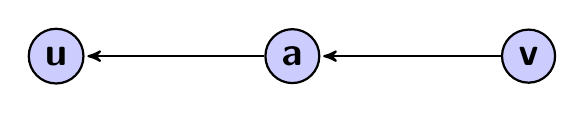
\begin{tikzpicture}[->,>=stealth',shorten >=1pt,auto,node distance=3cm,
        thick,main node/.style={circle,fill=blue!20,draw,font=\sffamily\Large\bfseries}]

        \node[main node] (1) {a};
        \node[main node] (2) [left of=1] {u};
        \node[main node] (4) [right of=1] {v};

        \path[every node/.style={font=\sffamily\small}]
        (4) edge node [left] {} (1)
        (1) edge node [right] {} (2);
      \end{tikzpicture}

      $u$ evidently has both incoming and outgoing edges in $G$.

      Consider a DFS run on the above counterexample directed graph $G$ starting from $a$ with the 
      following discovery and finish times.  

      \begin{center}
        \begin{tabular}{ l | c | r }
          \hline
            & $d$ & $f$ \\ \hline
          $a$ & 1 & 2 \\
          $v$ & 5 & 6 \\
          $u$ & 3 & 4 \\
          \hline  
        \end{tabular}
      \end{center}


      The DFS on $G$ will discover $a$ first then finish $a$. Then discover $u$, then finish $u$ since
      $a$ was discovered already. Finally DFS will discover $v$, then finish $v$.

      Thus, $u$ is neither an ancestor or a descendant of another vertex. The depth-first tree
      contains only $u$ with no descendants or ancestors. 

      Hence, the conjecture is disproved.

    %&=& &=& &=& &=& &=& &=& &=& &=& &=& &=& &=& &=& &=& &=& &=& =
    % Question 4 
    %&=& &=& &=& &=& &=& &=& &=& &=& &=& &=& &=& &=& &=& &=& &=& =
    \par
    \bigskip






  \end{enumerate}
\end{document}


